\documentclass[pdf,dvipsnames]{beamer}
\usepackage{xcolor}
\usepackage{colortbl}
\usepackage{epstopdf}
\usepackage{graphicx}
\usepackage{animate}
\usepackage{wrapfig}
\usenavigationsymbolstemplate{}
\usetheme{Singapore}
\graphicspath{ {../images/} }

\title{Bayesian Machine Learning}
\subtitle{}
\author{Roni Chikhmous}
\date{\today}

\begin{document}

%\AtBeginSection[]{
%\begin{frame}{Table of Contents}
%	\tableofcontents[currentsection]
%\end{frame}
%}

\begin{frame}
	\thispagestyle{empty}
	\titlepage
\end{frame}
\addtocounter{framenumber}{-1}

\section{Intro to Bayesian inference}

\subsection{Bayes' Theorem}

%%%%%%%%%%%%%%%%%%%%%%%%%%%%%%%%%
\newtheorem{bayesthm}{Bayes' Theorem}
\newtheorem{bayesrmk}{Remark}
\newtheorem{bayesexplained}{Breaking it down}
%%%%%%%%%%%%%%%%%%%%%%%%%%%%%%%%%
\begin{frame}{Let's get the formalities out of the way}
	\begin{bayesthm}
		\alt<1>{
		  $$P(A \mid B ) = \frac{P(B \mid A) \, P(A)}{P(B)}$$
		}{
			$${\color{red} P(}{\color{blue} A} \, {\color{red} \mid} \, {\color{orange} B}{\color{red} )} = 
			\frac{{\color{brown}P(B \mid A)} \, {\color{OliveGreen} P(A)}}{{\color{purple}P(B)}}$$
		}
	\end{bayesthm}
	\begin{bayesrmk}<1->
	Where A and B are events and $P(B) \neq 0$
	\end{bayesrmk}
	\begin{bayesexplained}<2->
	The {\color{red} chance} that a {\color{blue} hypothesis} is supported by {\color{orange} evidence} given the {\color{purple} chance of observing that evidence in general}, {\color{brown} the likelihood of obtaining it given the hypothesis} and {\color{OliveGreen} our prior beliefs}.
	\end{bayesexplained}
\end{frame}

\subsection{Illustrating the difference between Bayesian and frequentist reasoning}

\begin{frame}{Bayesian reasoning gives us the framework to define our uncertainty}
	This is the thinking process you're interested in:
	
	
	belief (prior) $\longrightarrow$ observe data (evidence) $\longrightarrow$ update prior $\longrightarrow$ get outcome (posterior)
	

	In frequentist approach, it doesn’t happen. You estimate maximum likelihood when given the data. The Bayesian approach is capturing our uncertainty about the quantity we are interested in. Maximum likelihood does not do this.


	As we get more and more data, the Bayesian and ML approaches agree more and more. However, Bayesian methods allow for a smooth transition from uncertainty to certainty.
\end{frame}

\begin{frame}{Consider looking for a ringing phone in one's apartment}
  \begin{wrapfigure}{r}{0.6\textwidth}
    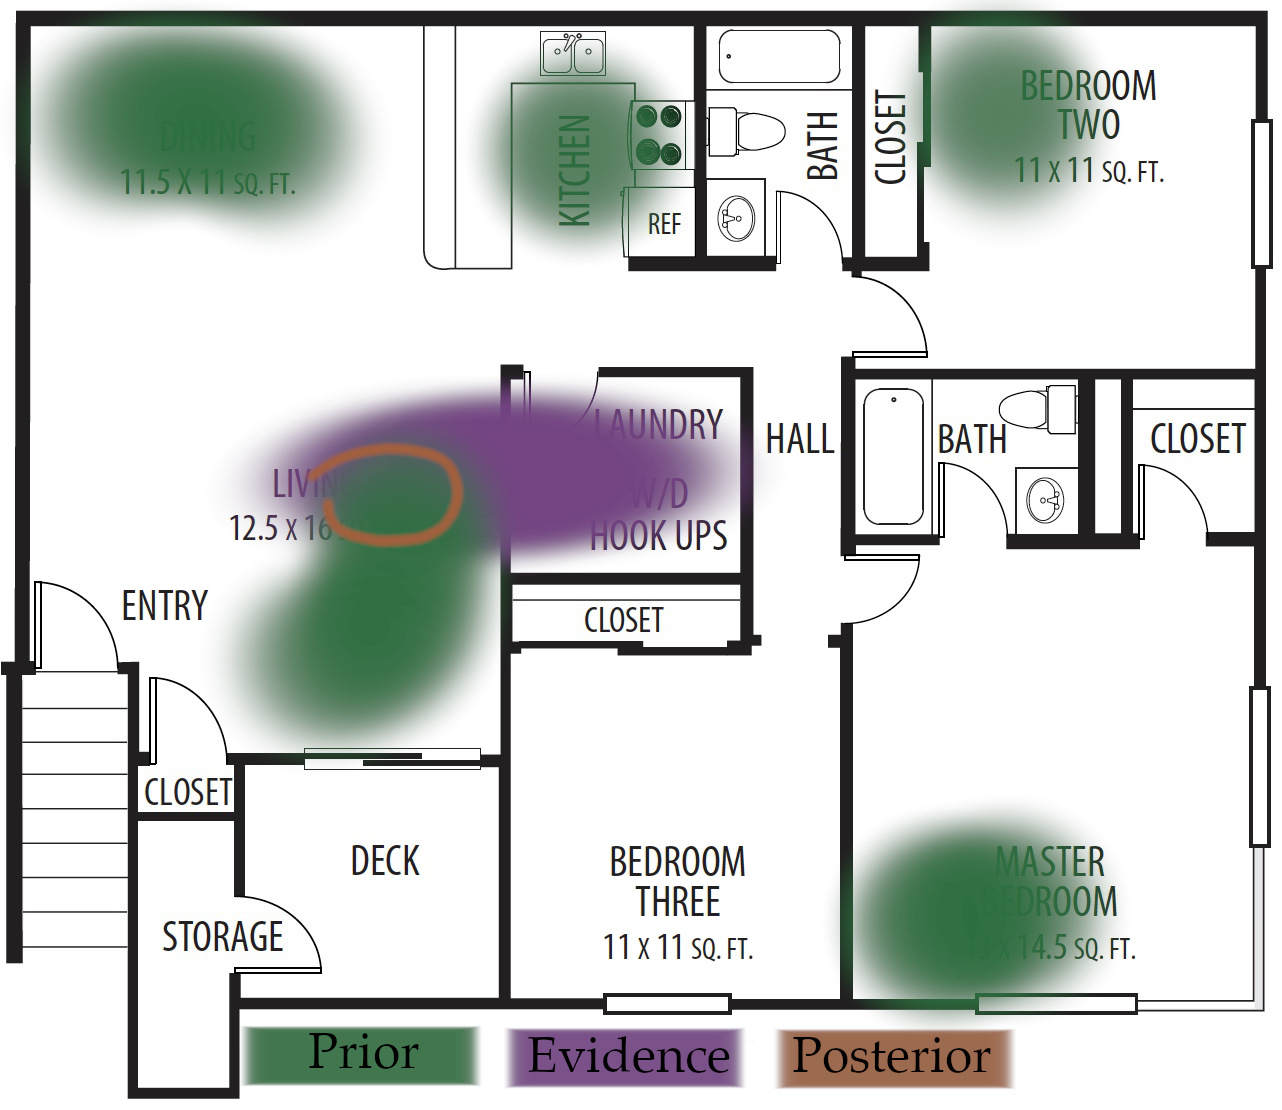
\includegraphics[width=0.55\textwidth,keepaspectratio]{apartment-plan}
	\end{wrapfigure}
  In that example:
  \begin{itemize}
  	\item you know where do you usually leave your phone (prior)
  	\item you hear where does the ringing come from (evidence)
  	\item you combine those two and go looking in the living room, instead of a laundry room\footnotemark (posterior)
  \end{itemize}
	\footnotetext[1]{Unless you have just finished doing laundry. But in that case your prior would be different.}
\end{frame}

\section{Workshop}

\begin{frame}{Let's flip some coins!}
	\begin{figure}
		\includegraphics{flipping-parrot-9}
	\end{figure}
\end{frame}

\end{document}

